\documentclass{article}
\usepackage{tikz}
\usetikzlibrary{automata}
\usetikzlibrary{graphs,shapes.geometric} 

\usepackage{graphicx, float, xcolor}
\usepackage{mathtools, mathrsfs, caption}
\usepackage{amsmath, amsfonts, amssymb, amsthm}
\captionsetup{font=small}

\usepackage{algorithm}
\usepackage[noend]{algpseudocode}
\newcommand\mycommfont[1]{\footnotesize\ttfamily\textcolor{blue}{#1}}
% \SetCommentSty{mycommfont}

% \SetKwInput{KwInput}{Input}                % Set the Input
% \SetKwInput{KwOutput}{Output}              % set the Output
\newcommand{\bigOh}[1]{\mathcal{O}(#1)}
\newcommand{\smallOh}[1]{\mathcal{o}(#1)}
\newcommand{\bigOmega}[1]{\Omega(#1)}
\newcommand{\smallomega}[1]{\omega(#1)}
\newcommand{\bigTheta}[1]{\Theta(#1)}

\usepackage{hyperref, biblatex}
\hypersetup{linkcolor=blue}
\usepackage[breakable,skins]{tcolorbox}
\tcbuselibrary{breakable}
\newcommand{\stepNumber}[1]{\textcolor{blue}{Step-(#1)}}
\usepackage{fancyhdr}
\pagestyle{fancy}
\chead{IEOR 6614: Homework 1}
\rhead{\textbf{UNI:} ag4808}
\lhead{02/12/24}

\begin{document}
\section{Problem 1}
If the weight of some edge in the original graph $G=(V, E)$ is decreased then the minimum spanning-tree (MST) may or may not change depending on, 
    \begin{enumerate}
        \item How much the edge weight is decreased by ?
        \item Whether the edge was in the original MST or not ?  
    \end{enumerate}
    \textbf{Case 1:} The edge $e = \{u, v\}$ has its weight reduced by $\delta > 0$ and $e \in T$, where $T$ is the MST for the original graph. We will prove that in this case the MST remains same. Assume that the MST for the new graph is some $T'\not=T$, then 
    \begin{itemize}
        \item \textbf{Case 1.1:} $e \in T'$, in this case $c'(T') = c(T')-\delta > c(T)-\delta = c'(T)$, which is a contradiction to the fact that $T'$ is an MST. 
        \item \textbf{Case 1.2:} $e \notin T'$, in this case $c'(T') = c(T') > c(T) > c'(T)$, which leads to similar contradiction as the previous case. 
        \item[] (notation: $c'(.)$ and $c(.)$ are cost-functions for the old and the new instance respectively)
    \end{itemize}
    Now we give two examples of graphs where $e\notin T$ and the resulting MST might change or not depending on the decrement value. Consider the graph $G = (V, E)$ as shown below, 
    \begin{figure}[H]
        \centering
        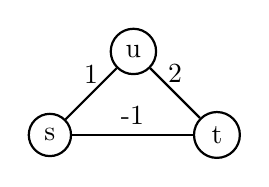
\begin{tikzpicture}[node distance={15mm}, thick, main/.style = {draw, circle}] 
            \node[main] (1) {s};
            \node[main] (2) [above right of = 1] {u}; 
            \node[main] (3) [below right of = 2] {t}; 

            \draw (1)--(2) node[midway, above] {1}; 
            \draw (2)--(3) node[midway, above] {2}; 
            \draw (3)--(1) node[midway, above] {-1}; 
        \end{tikzpicture}
        \caption{$G=(V, E)$, has a spanning tree $T = \{\{s, u\}, \{s, t\}\}$, $c(T)= 0$}
        \label{fig:sample graph}
    \end{figure}
    \noindent Note that, if we reduce the weight of the edge $e= \{u, t\}$ by $\delta = 0.5$ the MST remains the same but if we reduce by $\delta = 2$ the new MST is $T' = \{\{s, t\}, \{u, t\}\}$
    \begin{algorithm}[H]
        \caption{MOD-MST(T, e, $\delta$)}
        \begin{algorithmic}[1]
            \State $T' \leftarrow T + e$;
            \State $c(e) \leftarrow c(e) + \delta$; 
            \Statex
            \State Find a cycle $\Gamma$ in $T'$;
            \State Find $e^* = \arg\max_{e \in \Gamma} \{c(e)\}$; 
            \State Delete $e^*$ from $T'$ and return $T'$;  
        \end{algorithmic}
    \end{algorithm}
    \noindent \textbf{Claim :} If the edge $e = \{u, v\} \notin T$ is updated, then when added it forms a cycle $\Gamma$ in $T$, let $e^*$ be the most heavy edge of $\Gamma$. Then $T+e-e^*$ is the unique MST of the new graph. \\\\
    \textit{\underline{Proof-}} As the weight of $e$ is decreased by $\delta > 0$, and $e^*$ is the heaviest edge in $\Gamma$ (the existence and uniqueness of the cycle is guaranteed by properties of a MST). For all edges $f\not= e$ such that $f\notin T$, we know that $f$ will be the heaviest edge of some cycle in the old graph, as we modify only a single edge the same is true for the new graph too. Hence all such $f$ cannot be part of any MST. \\\\
    As any MST in the new graph cannot contain edges from $f$ and the edge $e^*$. The MST should be same as $T+e-e^* = T'$ (output of \stepNumber{5})\\\\
    \noindent \textbf{Claim :} The \texttt{MOD-MST} algorithm works in $\mathcal{O}(V)$ time.\\\\
    \textit{\underline{Proof -}} Assuming that adding, deleting an edge and updating weights can be done in constant time \stepNumber{1, 2, 5} take $\mathcal{O}(1)$ time. Now \stepNumber{3, 4} consist of finding $\Gamma$ and the heaviest edge of the cycle, which can be done via a breadth-first search which can be done in $\mathcal{O}(V+E)$, but as $T$ is a tree number of edges is linear in the number of vertices so the better bound is $\mathcal{O}(V)$
    \newpage
    \section{Problem 2}
    For the given vertices $t$ (target) and $s$ (source) find the $s-t$ path such that the maximum length of an edge on the path is the smallest, or more precisely if we define $b(\mathcal{P}) = \max_{e\in \mathcal{P}} c(e)$ as the bottleneck length of a $s-t$ path then, 
    \begin{equation*}
        \mathcal{P}^* = \arg\min_{\mathcal{P}} b(\mathcal{P})
    \end{equation*}
    Based on the above objective I propose the following modification in the shortest path algorithm we saw in the class. 
    \begin{algorithm}[H]
        \caption{MOD-DIJKSTRA(G, s, t)}
        \begin{algorithmic}[1]
            \State Mark all nodes $v\in V(G)$ as unvisited; 
            \State Label $b(s)\leftarrow -\infty$ and $b(v) \leftarrow \infty$ for all $v \in V(G)\setminus \{s\}$; 
            \State Mark $s$ as active; 
            \While{there is an unvisited vertex}
                \State Find $u^* = \arg \min_u b(u)$ such that $u^*$ is active and mark it visited. 
                \ForAll{$(u^*, v) \in E(G)$}
                    \State Mark $v$ as active if $v$ is not visited. 
                    \State Update $b(v) \leftarrow \min\{b(v), \max\{b(u^*), c(u^*, v)\}\}$
                \EndFor

            \EndWhile
            \Statex 
            \State \Return $b(t)$
        \end{algorithmic}
    \end{algorithm}
    \noindent Note that this algorithm has the same time-complexity analysis as the normal shortest-path version (depending on how we choose to implement with or without heaps, in the case of a min-heap we take $\bigOh{E\log V}$ time)\\\\
    \textbf{Claim :} The $\texttt{MOD-DIJKSTRA}$ algorithm correctly produces the shortest bottleneck path's (from $s$ to $t$) distance. \\\\
    \textit{\underline{Proof-}} Assume that $b(.)$ is maintained by a heap then at the start of each iteration (for the outer loop) we maintain the invariant that if the length of the smallest edge in the heap is $d$, then all the vertices of distance less than $d$ have been found and all the edges of weight larger than $d$ with one end as these vertices is in the heap. In each iteration of the algorithm we are just extracting the best value edge from the heap and determine the vertices that can be reached through that edge along the edges of less than or equal weight and maintain the invariant. (more or less we can also use the similar ideas as the proof of correctness for standard algorithm discussed in class with a changed greedy criterion). 
    \newpage
    \section{Problem 3}
    Let us consider the following network, 
    \begin{figure}[H]
        \centering
        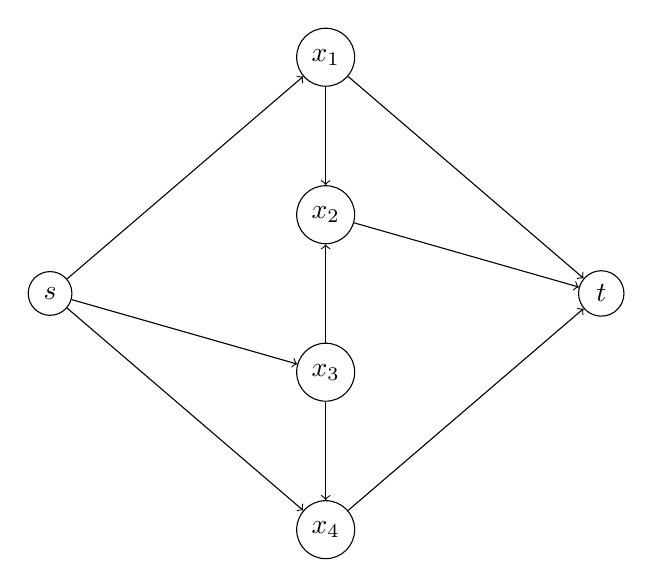
\begin{tikzpicture}
            \draw
            (-3, 0) node[circle, black, draw](s) {$s$} 
            (0.5, 3) node[circle, black, draw](x1) {$x_1$}
            (0.5, 1 )node[circle, black, draw](x2) {$x_2$}
            (0.5, -1) node[circle, black, draw](x3) {$x_3$}
            (0.5, -3) node[circle, black, draw](x4) {$x_4$}
            (4, 0) node[circle, black, draw](t) {$t$} ;

            \draw[->] (s)->(x1); 
            \draw[->] (s)->(x3); 
            \draw[->] (s)->(x4);
            \draw[->] (x1)->(t);
            \draw[->] (x2)->(t); 
            \draw[->] (x4)->(t); 
            \draw[->] (x1)->(x2); 
            \draw[->] (x3) -> (x2); 
            \draw[->] (x3) -> (x4); 
            
            
        \end{tikzpicture}
        \caption{Flow-network with single irrational capacities}
        \label{fig:flow network}
    \end{figure}
    The edge capacities are as follows (Let, $\sigma = (\sqrt{5}- 1)/2$), 
    \begin{itemize}
        \item $u(x_1, x_2) = \sigma$ (note that : $\sigma^n = \sigma^{n+1} + \sigma^{n+2}, \forall n \geq 0$)
        \item $u(x_3, x_2) = 1$
        \item $u(x_3, x_4) = 1$
        \item All other edges have capacity $M > 0$, where $M$ is a very large number. 
    \end{itemize}
    
    We start augmenting along the following sequence, 
    \begin{figure}[H]
        \centering
        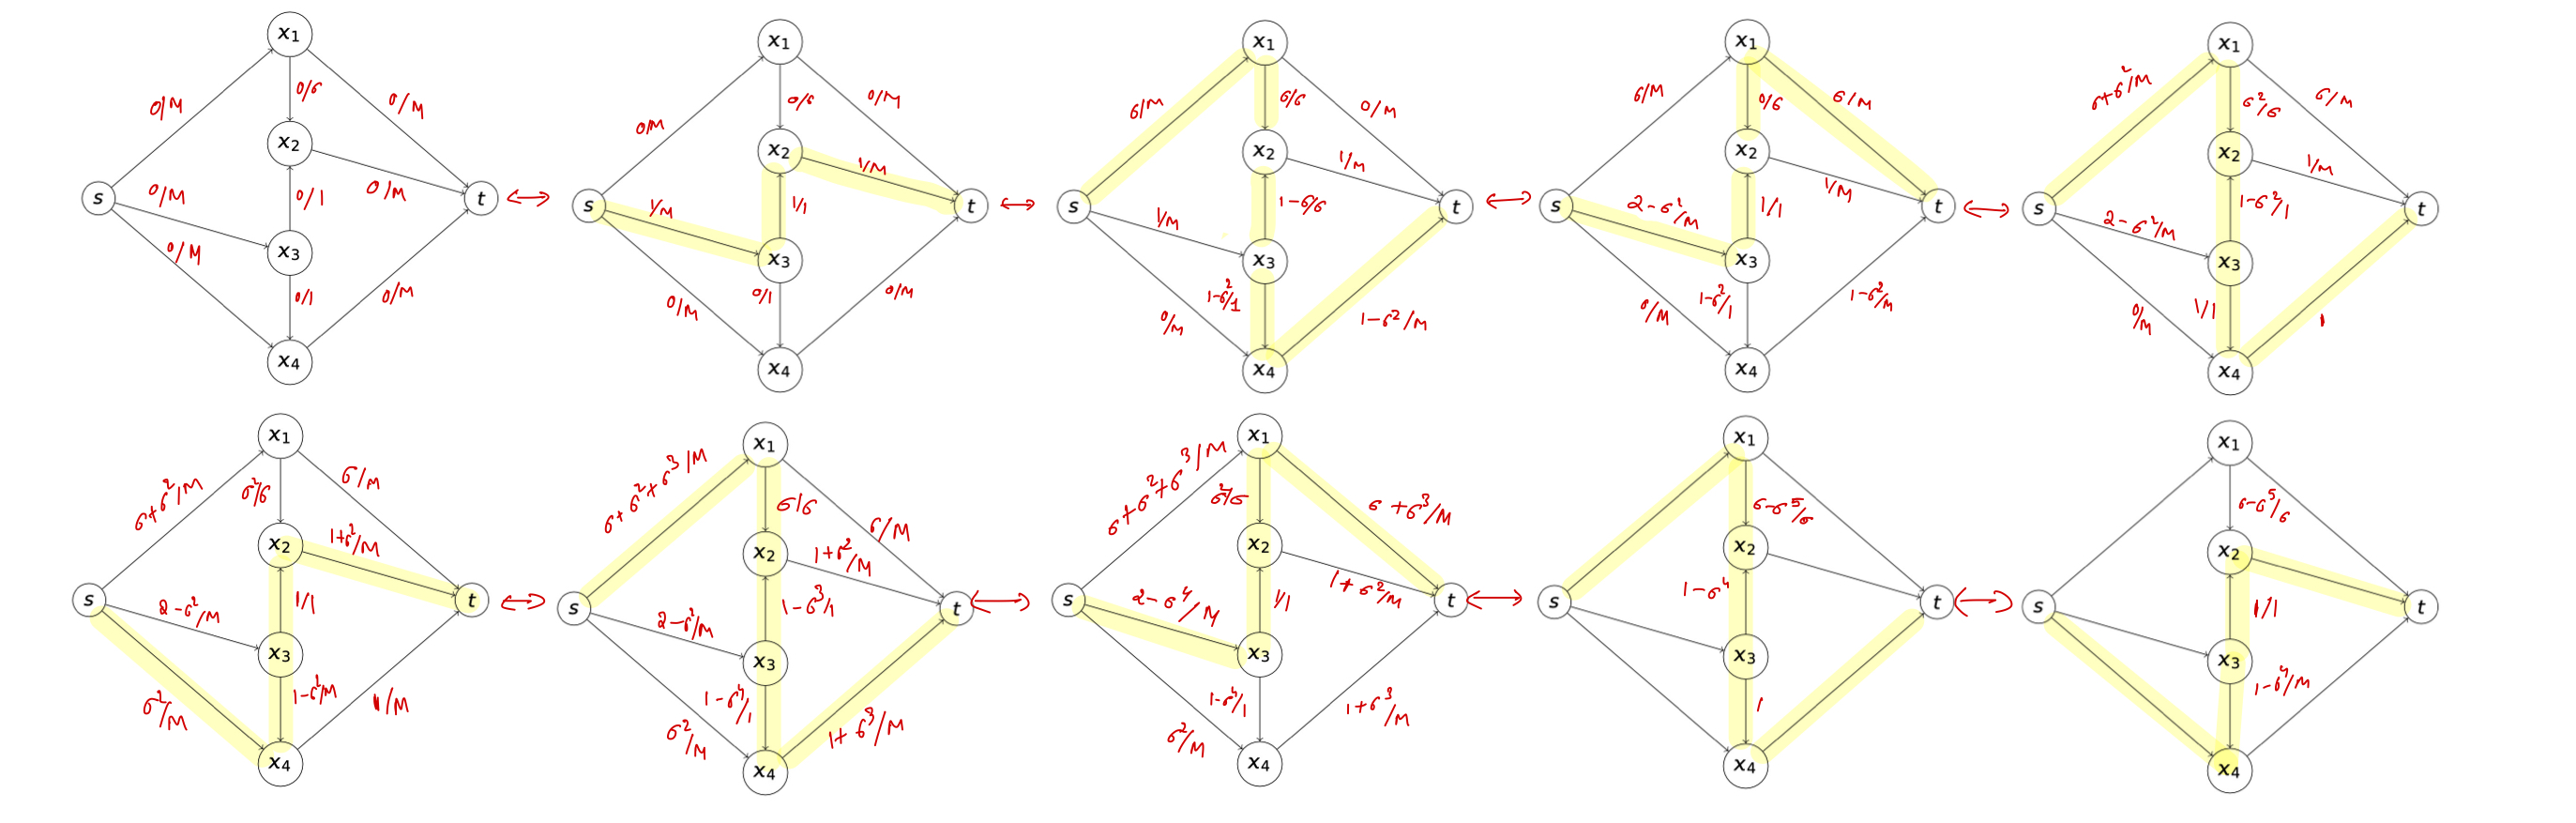
\includegraphics[width = \linewidth]{resources/HW1Q3.jpg}
        \caption{Sequence of augmenting paths \textcolor{blue}{[0-9]}}
        \label{fig:enter-label}
    \end{figure}
    \noindent Note the pattern, after $(4K+1)$ steps where $K\ge 0$ the flow-value is 
    \begin{equation*}
        \sum_{e\in \delta^+(s)} f_e = 1 + 2 \left(\sum_{k=1}^{K}\sigma^k\right)
    \end{equation*}
    \textbf{Note:} It can be seen that after the first augmentation, the flow is 1. For the following augmentations in the sequence we have a period of 4, in each period (say the $k^{th}$ period) for the first two augmentations we add $\sigma^k$ flow and for the last two we add $\sigma^{k+1}$. \\\\
    \textbf{Claim:} The Ford-Fulkerson algorithm may not terminate for the above sequence and max-flow found is incorrect.\\\\
    \textit{\underline{Proof-}} Using the given sequence of augmenting paths, every $(4K+1)^{th}$ path has the flow value, so after infinite such iterations: 
    \begin{equation*}
        f_\infty = \lim_{K\rightarrow \infty} 1 + 2 \left(\sum_{k=1}^{K}\sigma^k\right) = (3 + 2\sigma) < (2M+1)
    \end{equation*}
    Hence the sequence converges to $f_\infty$ which is less than the true max-flow after infinite iterations, and we are done. 
    \section{Problem 4}
    \textbf{Claim 1:} If $\Gamma$ is a circulation, then for any set $X\subset V$ we have, 
    \begin{equation*}
        \sum_{e \in \delta^+(X)} \Gamma(e) = \sum_{e \in \delta^-(X)} \Gamma(e)
    \end{equation*}
    \begin{proof}
        For each vertex $x\in X$, we have the flow conservation constraint for the circulation. Hence, 
        \begin{equation*}
            \sum_{e \in \delta^+(\{x\})} \Gamma(e) = \sum_{e \in \delta^-(\{x\})} \Gamma(e) \, \, \, \, \forall x \in X
        \end{equation*}
        If we sum these over all vertices $x \in X$, we get the following 
        \begin{equation*}
            \begin{split}
                \sum_{x \in X}\sum_{e \in \delta^+(\{x\})} \Gamma(e) &= \sum_{x \in X}\sum_{e \in \delta^-(\{x\})} \Gamma(e)\\
            \end{split}
        \end{equation*}
        \begin{equation*}
            \begin{split}
                \implies \sum_{e \in \delta^+(X)} \Gamma(e) + \sum_{e \in \gamma (X)} \Gamma(e) &= \sum_{e \in \delta^-(X)} \Gamma(e) + \sum_{e \in \gamma (X)} \Gamma(e)\\
                \implies \sum_{e \in \delta^+(X)} \Gamma(e) &= \sum_{e \in \delta^-(X)} \Gamma(e)
            \end{split}
        \end{equation*}
        Note, here $\gamma(X)$ defines all edges with both ends in $X$. \\\\
        \end{proof}
        \noindent \textbf{Claim 2:} If $\Gamma$ is a circulation then for all sets $X\subset V$ we have, 
        \begin{equation*}
            \sum_{e \in \delta^+(X)} u_e \ge \sum_{e \in \delta^-(X)} l_e 
        \end{equation*}
        \begin{proof}
            Note that for any set $X\subset V$ we have, 
            \begin{equation*}
                \sum_{e \in \delta^+(X)} \Gamma_e \le \sum_{e \in \delta^+(X)} u_e
            \end{equation*}
            \begin{equation*}
                \sum_{e \in \delta^-(X)} \Gamma_e \ge \sum_{e \in \delta^-(X)} l_e
            \end{equation*}
            Using the previous claim, we get that, 
            \begin{equation*}
                \sum_{e \in \delta^+(X)} u_e \ge \sum_{e \in \delta^+(X)} \Gamma_e = \sum_{e \in \delta^-(X)} \Gamma_e \ge \sum_{e \in \delta^-(X)} l_e
            \end{equation*}
            Which proves the necessary part of the Hoffman's circulation theorem. 
        \end{proof}
        \noindent To prove sufficiency we first define, 
        \begin{itemize}
            \item \textbf{Slack}: The slack of a vertex is defined as the difference between the outgoing and the incoming flow. It is denoted by $\Delta(.)$
            \item \textbf{Admissible Path}: A path is admissible if for each edge $e$ in the path, 
            \item[] \begin{itemize}
                        \item $f(e) < u(e)$, if $e$ is a forward edge. 
                        \item $f(e) > l(e)$, if $e$ is a forward edge. 
                    \end{itemize}
            \item[] Here $f(.)$ is the flow on the edge, $u(.)$ is the upper-bound and $l(e)$ is the lower-bound on the flow. 
        \end{itemize}
        I give a constructive procedure to convert a given flow into a circulation provided the necessary condition. 
        \begin{algorithm}[H]
            \caption{CIRCULATE($G, l, u$)}
            \begin{algorithmic}[1]
                \State Set for each $e\in E$, arbitrary flow obeying $l(e) \le f(e)\le u(e)$. 
                \State Calculate the slack $\Delta(v)$ for all vertices $v \in V$. 
                \While{$\exists v \in V : |\Delta(v)| > 0$}
                    \State Pick some vertex $v \in V$ with $\Delta(v) < 0$. 
                    \State Set $X$ as the set of all vertices reachable from $v$ via an admissible path
                    \State Pick some vertex $u \not= v$ in $X$ with $\Delta(u) > 0$, and call the path b/w them $\mathcal{P}(v, u)$
                    \State Find the maximum allowable increase (subject to cap.  constr.) on $\mathcal{P}(v, u)$ ($\gamma$)
                    \ForAll{$e \in \mathcal{P}(v, u)$}
                        \If{$e$ is a forward edge}
                            \State $f(e) \leftarrow f(e) + \gamma$
                        \EndIf
                        \State \textbf{else}
                        \State \indent $f(e) \leftarrow f(e) - \gamma$
                    \EndFor
                \EndWhile
                \Return $f$
            \end{algorithmic}
        \end{algorithm}
        \noindent \textbf{Claim 1:} After initialization in \stepNumber{1}, the sum of slacks for all vertices is zero. 
            \begin{proof}
                \begin{equation*}
                    \begin{split}
                        \sum_{v \in V} \Delta(v) &= \sum_{v \in V} \left(\sum_{e \in \delta^+(\{v\})} f(e) - \sum_{e \in \delta^-(\{v\})} f(e)\right)\\
                        &= 0 
                    \end{split}
                \end{equation*}
                The last equality is due to the fact, that for each edge's end-points the terms cancel. Using this claim, we are guaranteed that whatever the slacks might be they can't be all positive or negative. While $f$ is not a circulation, we can find some vertex with negative slack as in \stepNumber{4}
            \end{proof}
        \noindent \textbf{Claim 2:}  For a given $v$ if we define $X = \{u \in V \, | \, \mathcal{P}(v, u) \text{ is admissible}\}$, then
        \begin{equation*}
            \sum_{v \in X} \Delta(v) \ge 0 
        \end{equation*}
        \begin{proof}
            Note that if a vertex $x$ is not in $X$, then $f(e) = u(e)$ for all forward edges $e$ having one end-point in $X$ and other end-point as $x$. Similarly, $f(e) = l(e)$ for all reverse edges $e$ having one end-point as $x$ and other end-point in $X$. (this is trivially true by definition of admissible paths)\\\\
            Hence, summing the slacks over $X$, 
            \begin{equation*}
                \begin{split}
                    \sum_{v \in X} \Delta(v) &= \sum_{e \in \delta^+(X)} f(e) - \sum_{e \in \delta^-(X)} f(e)\\
                    &= \sum_{e \in \delta^+(X)} u(e) - \sum_{e \in \delta^-(X)} l(e)\\
                    &\ge 0 
                \end{split}
            \end{equation*}
            The last inequality is true as we have the given property for all $X\subseteq V$. This claim will help us establish that we can always find a $u$ for the given $v$ as in \stepNumber{6}. 
        \end{proof}
        \noindent \textbf{Claim 3:} For a given $v$ and $u$ found by the algorithm in \stepNumber{4, 6}, when we update the flow values on every edge on $\mathcal{P}(v, u)$ by $\gamma$, we reduce sum of absolute values of slacks over all vertices by $2\gamma$. 
        \begin{proof}
            For any valid $v$ and $u$, if we carry updates as in \stepNumber{9-12}, then for all the interior vertices in the path $P(v, u)$ the slack does not change as (similar to how we analyze Ford-Fulkerson), but for the vertex $v$ we have an increase in outflow of $\gamma$ and for vertex $u$ we have an increase of inflow of $\gamma$, which adds up to total decrement of $2\gamma$ in sum of absolute-slacks for all vertices. 
        \end{proof}
        \noindent Using the previous claim, we have established that in each iteration of the while-loop the sum of absolute-slacks decreases and hence the loop will terminate in finite-time with a feasible circulation. 
    \section{Problem 5}
    \begin{enumerate}
        \item At termination $\Delta = 1$, hence $G_f(\Delta)$ is nothing but the normal residual graph. As the algorithm terminates, there are no $s-t$ paths in the residual graph hence the output is a max-flow (as this condition is sufficient for max-flow, discussed in class). 
        \item As $\Delta = 2^{\lceil \log U \rceil}$, and in each iteration of the outer while loop we perform one scaling phase, we can say that number of scaling phases $\mathcal{P} \le \text{ number of iterations of outer while loop.}$ The number of iterations of the outer loop be $\mathcal{N}$ then 
        \begin{equation*}
            \begin{split}
                2^{\mathcal{N}} &= 2^{\lceil \log U \rceil}\\
                \implies & \mathcal{N} = \lceil \log U \rceil\\
                \implies & \mathcal{N} = \bigOh{\log U}
            \end{split}
        \end{equation*}
        Hence, $\mathcal{P} = \bigOh{\log U}$
        \item At the end of any $\Delta$-scaling phase, there are no s-t paths in $G_f(\Delta)$ thus there must be some $s-t$ cut $(L, R)$ such that each arc in $\delta^+(L)$ has residual capacity less than $\Delta$. This implies that the residual capacity of the cut is at most $m\Delta$ at the end of this phase.
        \item \textbf{Claim:} If $f$ is an $s-t$ flow in $G$, and $f^*$ is the max-flow in $G$ then the max-flow in the residual graph is $|f^*|-|f|$. 
        \item[] \textit{\underline{Proof -}} We first prove an additional claim. Consider $f'' = f^* - f$, we need to show that $f''$ is a flow in the residual network. Note as both $f^*$ and $f$ are flows we know that flow conservation holds. For capacity constraints note that $f''(i, j) = f^*(i, j) - f(i, j)\le u(i, j) - f(i, j) = u_f(i, j)$, i.e. - the residual capacity. The value of $f''$ in the residual network is $|f^*|-|f|$. To show it is the max-flow consider a minimum $s-t$ cut $S$ in $G$ so that $|f^*| = u(\delta^+(S))$ then for each arc in $\delta^+(S)$ we have $f^*(i, j) = u(i, j)$ and hence $f''(i, j) = u_f(i, j)$. So $|f''| = u_f(\delta^+(S))$, and we are done. 
        \item[]At each iteration in the $\Delta$-scaling phase the value of the flow increases by at least $\Delta$ (as each $s-t$ path has residual capacity at least $\Delta$, pushing flow along the path will increase the flow value by at least $\Delta$). Let $f$be the flow at the beginning of the $\Delta$-scaling phase, and let $f^*$ be a max-flow. Then by the previous part and the claim above, $|f^*| -|f| \le 2m \Delta$. Thus in $2m$ iterations the value of the resulting flow must be at least $|f| +2m\Delta \le |f| + |f^*|-|f| = |f^*|$, so the flow must be maximum and no further augmenting paths can be found. 
        \item From the parts (b) and (d) we can see that we have a $\bigOh(\log U)$ scaling phases and each scaling phase has $\bigOh{m}$ augmentations and each augmentation can take $\bigOh{m}$ constant time operations so we have a total time complexity of $\bigOh{m^2\log U}$
    \end{enumerate}
    \section{Problem 6}
        Let us denote the set of all flights by $\mathcal{F}$, and each flight $f \in \mathcal{F}$ is denoted by a tuple $f = \langle o_f, d_f, s_f, e_f\rangle$ where, 
        \begin{enumerate}
            \item $o_f$: is the origin of the flight 
            \item $d_f$: is the destination of the flight
            \item $s_f$: is the starting time for the flight from $o_f$. 
            \item $e_f$: is the arrival time for the flight on $d_f$. 
        \end{enumerate}
        Two flights $f$ and $f'$ can be served by a single plane if $d_f = o_{f'}$ and $s_{f'} \leq e_{f}$. The objective is to find the minimum number of planes required to serve $\mathcal{F}$, Note that we should be able to serve any $\mathcal{F}$ with at most $|\mathcal{F}|$ planes (one for each flight in the worst case).\\\\
        \textbf{Reduction Graph:}\\\\
        For a given number of planes $k$, 
        \begin{enumerate}
            \item Add a source node $s$ and a sink node $t$. 
            \item For each flight $f\in \mathcal{F}$ add two nodes $o_f$ and $d_f$ corresponding to the origin and the destination. 
            \item For each arc $(o_f, d_f)$ put a lower bound = 1, upper bound = 1 on the flow value. 
            \item For each arc $(s, o_f)$ put a lower bound = 0, upper bound = 1 on the flow value. 
            \item For each arc $(d_f, t)$ put a lower bound = 0, upper bound = 1 on the flow value. 
            \item Add an edge $(s, t)$ with a lower bound = 0 and an upper bound = $k$. 
            \item Add an edge $(t, s)$ with a lower bound = $k$ and an upper bound = $k$. 
        \end{enumerate}
        We want to show that if a circulation exists in the above flow network for a given value of $k$, then we have a feasible schedule with $k$ planes. We first convert this flow network with lower bounds to a flow network with demands and zero-lower bounds.\\\\
        \textbf{Conversion 1:}
        \begin{itemize}
            \item Send in a flow equal to lower bound on each edge. 
            \item $e = (u, v)$ had a lower bound $l(e)$, then the demand of $u$ is $l(e)$ and demand of $v$ is $-l(e)$. 
        \end{itemize}
        We reduce this further to the conventional max-flow problem as circulations are more general and we do not have appropriate algorithms for them.\\\\
        \textbf{Conversion 2:}
        \begin{enumerate}
            \item Add a source node $S$, and a sink node $T$. 
            \item For each $v$ with demand $d(v) < 0$, add edge $(S, v)$ with capacity $-d(v)$
            \item For each $v$ with demand $d(v) > 0$, add edge $(v, T)$ with capacity $d(v)$
        \end{enumerate}
        We claim that a circulation in the network after conversion-1 exists iff the max-flow in the network after conversion-2 is $\sum_{v:d(v)>0} d(v)$. But before proving the two claims, we lay down the algorithm assuming these claims to be true and analyze the runtime. 
        \begin{algorithm}[H]
            \caption{SCHEDULE ($\mathcal{F}$)}
            \begin{algorithmic}[1]
                \ForAll{$k = 1, \dots, |\mathcal{F}|$}
                    \State Perform reduction. 
                    \State Perform conversion 1. 
                    \State Perform conversion 2. 
                    \State Solve Max-Flow, and check the condition of conversion 2. 
                    \State If yes, break and return $k$.
                \EndFor
            \end{algorithmic}
        \end{algorithm}
        Note, the graph formed has $\bigOh{|\mathcal{F}|}$ vertices and $\bigOh{|\mathcal{F}|^2}$ edges. We solve at worst  $\bigOh{|\mathcal{F}|}$ problems, and each max-flow problem requires  $\bigOh{|\mathcal{F}|}$ augmentations. Hence the overall complexity is $\bigOh{|\mathcal{F}|^4}$. It is not the tightest bound as an immediate improvement can be found if we employ a binary search over $k$, which improves it to $\bigOh{|\mathcal{F}|^3 \log |\mathcal{F}|}$\\\\
        For a proof of conversion-2 note that if we define $\sum_{v:d(v)>0} d(v) = D$, then there cannot be a $S-T$ flow in the new graph having value greater than $D$ as the cut $(A, B)$ with $A= \{s\}$ has capcity $D$. Now if there is a feasible circulation $f$ with demands $\{d(v)\}$ in the original graph then by sending a flow value of $-d(v)$ on each edge $(S, v)$ and a flow value of $d(v)$ on each edge $(v, T)$ we obtain a $S-T$ flow in the new graph of value $D$, and so it is a max-flow. Conversely, suppose that there is a max $S-T$ flow in the new graph of value $D$. Then each edge out of $S$ and each edge into $T$ must be saturated with flow. Thus if we delete these edges, we obtain a circulation in the original graph.\\\\
        For a proof of conversion-1 note that, let $f'$ be a circulation in the new graph. Define a circulation $f$ in the old graph by $f = f' + l$. Then $f$ satisfies the capacity conditions of the old graph. Also, 
        \begin{equation*}
            \begin{split}
                f_{in}(v) - f_{out}(v) &= \sum_{e \in \delta^-(\{v\})} (l_e + f'(e)) - \sum_{e \in \delta^+(\{v\})} (l_e + f'(e))\\
                &= d(v)
            \end{split}
        \end{equation*}
        Hence demand conditions are met. For the other side of the proof, assume that $f$ is a circulation in the old graph, define a circulation $f'$ in the new graph by $f' = f - l$. Then on checking the capacity and the conservation constraints analogously we are done. 
    \section{Problem 7}
    We have the input graph $G = (V, E)$. Suppose after solving the global min-cut problem we get two sets of vertices $A$ and $B$. Assume that there is a poly-time subroutine to solve the minimum $s-t$ cut problem, then if we pick some arbitrary vertex $s$, and the global min-cut is $(A, B)$ such that $A, B\not=\varphi$ then it must separate $s$ from some vertex $t \in V$ not same as $s$. We can use this idea for a reduction base algorithm. 
    \begin{algorithm}[H]
        \caption{Global-MinCut(G)}
        \begin{algorithmic}[1]
            \State Pick some $u \in V$. 
            \State $c \leftarrow \infty$
            \ForAll{$v\not=u \, \& v \in V$}
            \State Compute the $u-v$ min-cut value $c_{uv}$
            \If{$c_{uv} \le c$} 
                \State $c \leftarrow c_{uv}$
            \EndIf
            \EndFor
            \Return $c$
        \end{algorithmic}
    \end{algorithm}
    \noindent \textbf{Runtime:} We assume a poly-time subroutine for solving a single instance of min-cut problem (like Ford-Fulkerson etc.) We essentially use this routine $(|V|-1)$ times (one time for each vertex $v\not= u$). Hence we solve $\bigTheta{V}$ min-cut problems. \\\\
    \textbf{Correctness :}
    \begin{itemize}
        \item Solving the minimum cut problem in the residual-graph $G_r$ is the same
as the minimum cut in an un-directed graph G. There are three types of directed edges in $G_r$ :
    \begin{enumerate}
        \item Type-A: edge from a vertex in $A$ to a vertex in $B$
        \item Type-B: edge from a vertex in $B$ to a vertex in $A$
        \item Type-C: edges that are internal to sets $A$ and $B$
    \end{enumerate}
    If a source is fixed in A and the sink in B, the minimum cut in the
    residual graph $G_r$ will have only Type-A edges. The Type-B edges will
    not be part of the minimum cut. The minimum cut in the residual
    graph $G_r$ will contain only Type-1 edges from $A$ to $B$, which corresponds to the cut separating the two sets A and B in the original graph
    $G$. The argument can be reversed for the cases when the source is fixed
    in $B$ and the sink in $A$. This minimum cut edge set of $G_r$ will be the
    same as the min-cut edge set of $G$ as, there too we’ll have the same
    edge set of undirected edges with one end in $A$ and the other in $B$
    
    \item To prove that we end up with the correct global minimum cut, it is enough to prove that we’d obtain the same minimum cut for any source vertex $x \in A$ and sink vertex $y \in B$, i.e. the global minimum cut remains same for all choice of $x$ and $y$. This would be true since the minimum cut of $G$ represents a frontier that needs to be crossed to get from any vertex in $A$ to any vertex in $B$. For any other $x' \in A$ and $y' \in B$, the same minimum cut holds in any undirected Graph $G$. Conversely, if it did not then, the minimum cut for $x$ and $y$ would also change given that $x$ and $x'$ are in the same set and $y$ and $y'$ are in the same set. Therefore, the same minimum cut holds irrespective of the choice of $x$ and $y$. Any variation from this would imply a discrepancy in the separation of sets $A$ and $B$ in the original undirected graph $G$
    \end{itemize}
    \section{Problem 8}
    Let us define the capacity function $u'_k : E\rightarrow \mathbb{Z}_{\ge 0}$ for a given $ k \ge 1$ as follows, 
    \begin{equation*}
        u'(e) = k|E|u(e) + 1, \, \, \, \, \, \forall e \in E
    \end{equation*}
    \textbf{Claim:} Running max-flow algorithm on the new instance produces the min-cut with minimum number of edges. 
    \begin{proof}
        Let $X\subset V$ be a non-empty set then the min-cut $X^*$ is given by, 
        \begin{equation*}
            \begin{split}
                X^* &= \arg \min_{X} u^+(X)\\
                &= \arg \min_{X} \sum_{e \in \delta^+(X)}k|E|u(e) + 1\\
                &= \arg \min_{X} \left( k|E|\left(\sum_{e \in \delta^+(X)}u(e)\right) + |\delta^+(X)|\right)
            \end{split}
        \end{equation*}
        If we consider any cut-set $A$, which was not the min-cut for the original instance and any cut-set $A^*$ which was the min-cut then  if we define $f(X) = k|E|\left(\sum_{e \in \delta^+(X)}u(e)\right) + |\delta^+(X)|$, then $f(A) > f(A^*)$. 
        \begin{equation*}
            f(A) - f(A^*) = k|E|\Delta_1 + \Delta_2
        \end{equation*}
        Here $\Delta_1 =\sum_{e \in \delta^+(A)}u(e) - \sum_{e \in \delta^+(A^*)}u(e) \ge 1$ and $\Delta_2 = |\delta^+(A)| - |\delta^+(A^*)| \ge (1-|E|)$, adding these two up we get $f(A)-f(A^*) \ge (k-1)|E| + 1 > 0$. Hence no sub-optimal cut of the original instance is the min-cut for the new instance.\\\\
        Moreover, amongst all the min-cuts of the original instance the new instance will pick the one with minimum value of $|\delta^+(X)|$, as the other part of the objective will be the same, hence satisfying our purpose. 
    \end{proof}
\end{document}
